After successfully building the voltage regulator circuit shown in
Figure~\ref{fig:schem1}, an oscilloscope was used to compare the input and
output waveforms.  As screen capture showing these signals (offset in the image
for clarity), as well as the RMS value of the input and average of the output.
%
\begin{figure}[H]
	\centering
	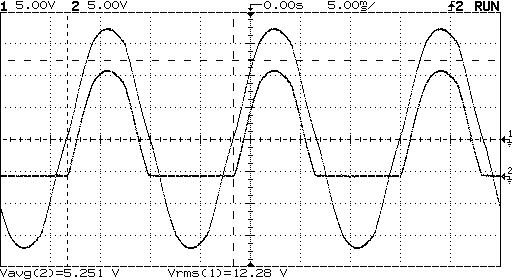
\includegraphics[width=4.25in]{img/ss1.png}
	\parbox{4.25in}{\caption{Oscilloscope screenshot of the completed half-wave rectifier
		outlined in Figure~\ref{fig:schem1}.  Signal one is the input, whereas
		signal two is the output across the resistor.}
	\label{fig:ck1plot}}
\end{figure}
%
The circuit was intially designed for an input of~\SI{12.2}{\volt} RMS and an
average output of~\SI{5.6}{\volt}.  As is shown, the input of~\SI{12.28}{\volt}
RMS is well within reasonable expectations of accuracy.  The measured output
of~\SI{5.251}{\volt}, while lower than expected, is still within reasonable
limits, as it is just~6.23\% below the designed value.  Inconsistencies with
the variac transformer and a resistance that was slightly below its
rated~\SI{1}{\kilo\ohm} likely contributed to this, along with small
capacitances in the oscilloscopes.

\begin{figure}[H]
	\centering
	\begin{tikzpicture}[gnuplot]
%% generated with GNUPLOT 4.4p2 (Lua 5.1.4; terminal rev. 97, script rev. 96a)
%% Wed 28 Sep 2011 01:27:40 PM EDT
\gpsolidlines
\gpcolor{gp lt color border}
\gpsetlinetype{gp lt border}
\gpsetlinewidth{1.00}
\draw[gp path] (1.320,0.985)--(1.500,0.985);
\node[gp node right] at (1.136,0.985) { 4};
\draw[gp path] (1.320,1.608)--(1.500,1.608);
\node[gp node right] at (1.136,1.608) { 5};
\draw[gp path] (1.320,2.231)--(1.500,2.231);
\node[gp node right] at (1.136,2.231) { 6};
\draw[gp path] (1.320,2.854)--(1.500,2.854);
\node[gp node right] at (1.136,2.854) { 7};
\draw[gp path] (1.320,3.477)--(1.500,3.477);
\node[gp node right] at (1.136,3.477) { 8};
\draw[gp path] (1.320,4.100)--(1.500,4.100);
\node[gp node right] at (1.136,4.100) { 9};
\draw[gp path] (1.320,4.723)--(1.500,4.723);
\node[gp node right] at (1.136,4.723) { 10};
\draw[gp path] (1.320,5.346)--(1.500,5.346);
\node[gp node right] at (1.136,5.346) { 11};
\draw[gp path] (1.320,0.985)--(1.320,1.165);
\node[gp node center] at (1.320,0.677) { 5};
\draw[gp path] (3.551,0.985)--(3.551,1.165);
\node[gp node center] at (3.551,0.677) { 10};
\draw[gp path] (5.781,0.985)--(5.781,1.165);
\node[gp node center] at (5.781,0.677) { 15};
\draw[gp path] (8.012,0.985)--(8.012,1.165);
\node[gp node center] at (8.012,0.677) { 20};
\draw[gp path] (10.242,0.985)--(10.242,1.165);
\node[gp node center] at (10.242,0.677) { 25};
\draw[gp path] (1.320,5.346)--(1.320,0.985)--(10.242,0.985);
\node[gp node center,rotate=-270] at (0.246,3.165) {Output Voltage, $V_{out}$ (V)};
\node[gp node center] at (5.781,0.215) {Input Voltage, $V_{in}$ (V)};
\gpcolor{gp lt color 0}
\gpsetlinetype{gp lt plot 0}
\draw[gp path] (1.320,1.606)--(1.766,2.229)--(2.212,2.853)--(2.658,3.476)--(3.104,4.099)%
  --(3.551,4.568)--(3.997,4.605)--(4.443,4.630)--(4.889,4.686)--(5.335,4.734)--(5.781,4.778)%
  --(6.227,4.821)--(6.673,4.866)--(7.119,4.917)--(7.565,4.965)--(8.012,4.997)--(8.458,4.966)%
  --(8.904,4.929)--(9.350,4.890)--(9.796,4.847)--(10.242,4.810);
\gpsetpointsize{4.00}
\gppoint{gp mark 1}{(1.320,1.606)}
\gppoint{gp mark 1}{(1.766,2.229)}
\gppoint{gp mark 1}{(2.212,2.853)}
\gppoint{gp mark 1}{(2.658,3.476)}
\gppoint{gp mark 1}{(3.104,4.099)}
\gppoint{gp mark 1}{(3.551,4.568)}
\gppoint{gp mark 1}{(3.997,4.605)}
\gppoint{gp mark 1}{(4.443,4.630)}
\gppoint{gp mark 1}{(4.889,4.686)}
\gppoint{gp mark 1}{(5.335,4.734)}
\gppoint{gp mark 1}{(5.781,4.778)}
\gppoint{gp mark 1}{(6.227,4.821)}
\gppoint{gp mark 1}{(6.673,4.866)}
\gppoint{gp mark 1}{(7.119,4.917)}
\gppoint{gp mark 1}{(7.565,4.965)}
\gppoint{gp mark 1}{(8.012,4.997)}
\gppoint{gp mark 1}{(8.458,4.966)}
\gppoint{gp mark 1}{(8.904,4.929)}
\gppoint{gp mark 1}{(9.350,4.890)}
\gppoint{gp mark 1}{(9.796,4.847)}
\gppoint{gp mark 1}{(10.242,4.810)}
\gpcolor{gp lt color border}
\gpsetlinetype{gp lt border}
\draw[gp path] (1.320,5.346)--(1.320,0.985)--(10.242,0.985);
%% coordinates of the plot area
\gpdefrectangularnode{gp plot 1}{\pgfpoint{1.320cm}{0.985cm}}{\pgfpoint{10.242cm}{5.346cm}}
\end{tikzpicture}
%% gnuplot variables

	\parbox{4.25in}{
	\caption{Output of the zener diode-based voltage regulator shown in
		Figure~\ref{fig:schem3}, as measured on a DC voltmeter.  A 1N4740 diode
		was used in this test.}
	\label{fig:ckt3plot}}
\end{figure}

\begin{figure}[H]
	\centering
	\begin{tikzpicture}[gnuplot]
%% generated with GNUPLOT 4.4p2 (Lua 5.1.4; terminal rev. 97, script rev. 96a)
%% Wed 28 Sep 2011 10:44:45 AM EDT
\gpsolidlines
\gpcolor{gp lt color border}
\gpsetlinetype{gp lt border}
\gpsetlinewidth{1.00}
\draw[gp path] (1.504,0.985)--(1.684,0.985);
\node[gp node right] at (1.320,0.985) { 3};
\draw[gp path] (1.504,1.619)--(1.684,1.619);
\node[gp node right] at (1.320,1.619) { 3.5};
\draw[gp path] (1.504,2.253)--(1.684,2.253);
\node[gp node right] at (1.320,2.253) { 4};
\draw[gp path] (1.504,2.888)--(1.684,2.888);
\node[gp node right] at (1.320,2.888) { 4.5};
\draw[gp path] (1.504,3.522)--(1.684,3.522);
\node[gp node right] at (1.320,3.522) { 5};
\draw[gp path] (1.504,4.156)--(1.684,4.156);
\node[gp node right] at (1.320,4.156) { 5.5};
\draw[gp path] (1.504,4.790)--(1.684,4.790);
\node[gp node right] at (1.320,4.790) { 6};
\draw[gp path] (1.504,0.985)--(1.504,1.165);
\node[gp node center] at (1.504,0.677) { 0};
\draw[gp path] (2.378,0.985)--(2.378,1.165);
\node[gp node center] at (2.378,0.677) { 0.5};
\draw[gp path] (3.252,0.985)--(3.252,1.165);
\node[gp node center] at (3.252,0.677) { 1};
\draw[gp path] (4.125,0.985)--(4.125,1.165);
\node[gp node center] at (4.125,0.677) { 1.5};
\draw[gp path] (4.999,0.985)--(4.999,1.165);
\node[gp node center] at (4.999,0.677) { 2};
\draw[gp path] (5.873,0.985)--(5.873,1.165);
\node[gp node center] at (5.873,0.677) { 2.5};
\draw[gp path] (6.747,0.985)--(6.747,1.165);
\node[gp node center] at (6.747,0.677) { 3};
\draw[gp path] (7.621,0.985)--(7.621,1.165);
\node[gp node center] at (7.621,0.677) { 3.5};
\draw[gp path] (8.494,0.985)--(8.494,1.165);
\node[gp node center] at (8.494,0.677) { 4};
\draw[gp path] (9.368,0.985)--(9.368,1.165);
\node[gp node center] at (9.368,0.677) { 4.5};
\draw[gp path] (10.242,0.985)--(10.242,1.165);
\node[gp node center] at (10.242,0.677) { 5};
\draw[gp path] (1.504,4.790)--(1.504,0.985)--(10.242,0.985);
\node[gp node center,rotate=-270] at (0.246,2.887) {Measured Current, $I_{out}$ (\si{\milli\ampere})};
\node[gp node center] at (5.873,0.215) {Load Resistance, $R$ (\si{\kilo\ohm})};
\node[gp node center] at (5.873,5.252) {Measured current from a JFET-based constant current source};
\node[gp node right] at (3.712,1.627) {16V source};
\gpcolor{gp lt color 0}
\gpsetlinetype{gp lt plot 0}
\draw[gp path] (3.896,1.627)--(4.812,1.627);
\draw[gp path] (1.591,4.384)--(1.679,4.371)--(1.854,4.371)--(2.028,4.371)--(2.203,4.371)%
  --(2.378,4.384)--(2.553,4.384)--(2.727,4.384)--(2.902,4.384)--(3.077,4.384)--(3.252,4.384)%
  --(3.426,4.384)--(3.601,4.384)--(3.776,4.384)--(3.951,4.397)--(4.125,4.397)--(4.300,4.384)%
  --(4.475,4.371)--(4.650,4.346)--(4.824,4.333)--(4.999,4.333)--(5.174,4.308)--(5.349,4.245)%
  --(5.523,4.169)--(5.698,4.067)--(5.873,3.940)--(6.048,3.801)--(6.223,3.648)--(6.397,3.496)%
  --(6.572,3.331)--(6.747,3.179)--(6.922,3.027)--(7.096,2.875)--(7.271,2.735)--(7.446,2.608)%
  --(7.621,2.469)--(7.795,2.342)--(7.970,2.228)--(8.145,2.101)--(8.320,1.987)--(8.494,1.886)%
  --(8.669,1.784)--(8.844,1.683)--(9.019,1.581)--(9.193,1.492)--(9.368,1.404)--(9.543,1.327)%
  --(9.718,1.239)--(9.892,1.163)--(10.067,1.086)--(10.242,1.010);
\gpsetpointsize{4.00}
\gppoint{gp mark 1}{(1.591,4.384)}
\gppoint{gp mark 1}{(1.679,4.371)}
\gppoint{gp mark 1}{(1.854,4.371)}
\gppoint{gp mark 1}{(2.028,4.371)}
\gppoint{gp mark 1}{(2.203,4.371)}
\gppoint{gp mark 1}{(2.378,4.384)}
\gppoint{gp mark 1}{(2.553,4.384)}
\gppoint{gp mark 1}{(2.727,4.384)}
\gppoint{gp mark 1}{(2.902,4.384)}
\gppoint{gp mark 1}{(3.077,4.384)}
\gppoint{gp mark 1}{(3.252,4.384)}
\gppoint{gp mark 1}{(3.426,4.384)}
\gppoint{gp mark 1}{(3.601,4.384)}
\gppoint{gp mark 1}{(3.776,4.384)}
\gppoint{gp mark 1}{(3.951,4.397)}
\gppoint{gp mark 1}{(4.125,4.397)}
\gppoint{gp mark 1}{(4.300,4.384)}
\gppoint{gp mark 1}{(4.475,4.371)}
\gppoint{gp mark 1}{(4.650,4.346)}
\gppoint{gp mark 1}{(4.824,4.333)}
\gppoint{gp mark 1}{(4.999,4.333)}
\gppoint{gp mark 1}{(5.174,4.308)}
\gppoint{gp mark 1}{(5.349,4.245)}
\gppoint{gp mark 1}{(5.523,4.169)}
\gppoint{gp mark 1}{(5.698,4.067)}
\gppoint{gp mark 1}{(5.873,3.940)}
\gppoint{gp mark 1}{(6.048,3.801)}
\gppoint{gp mark 1}{(6.223,3.648)}
\gppoint{gp mark 1}{(6.397,3.496)}
\gppoint{gp mark 1}{(6.572,3.331)}
\gppoint{gp mark 1}{(6.747,3.179)}
\gppoint{gp mark 1}{(6.922,3.027)}
\gppoint{gp mark 1}{(7.096,2.875)}
\gppoint{gp mark 1}{(7.271,2.735)}
\gppoint{gp mark 1}{(7.446,2.608)}
\gppoint{gp mark 1}{(7.621,2.469)}
\gppoint{gp mark 1}{(7.795,2.342)}
\gppoint{gp mark 1}{(7.970,2.228)}
\gppoint{gp mark 1}{(8.145,2.101)}
\gppoint{gp mark 1}{(8.320,1.987)}
\gppoint{gp mark 1}{(8.494,1.886)}
\gppoint{gp mark 1}{(8.669,1.784)}
\gppoint{gp mark 1}{(8.844,1.683)}
\gppoint{gp mark 1}{(9.019,1.581)}
\gppoint{gp mark 1}{(9.193,1.492)}
\gppoint{gp mark 1}{(9.368,1.404)}
\gppoint{gp mark 1}{(9.543,1.327)}
\gppoint{gp mark 1}{(9.718,1.239)}
\gppoint{gp mark 1}{(9.892,1.163)}
\gppoint{gp mark 1}{(10.067,1.086)}
\gppoint{gp mark 1}{(10.242,1.010)}
\gppoint{gp mark 1}{(4.354,1.627)}
\gpcolor{gp lt color border}
\node[gp node right] at (3.712,1.319) {32V source };
\gpcolor{gp lt color 1}
\gpsetlinetype{gp lt plot 1}
\draw[gp path] (3.896,1.319)--(4.812,1.319);
\draw[gp path] (1.591,4.004)--(1.679,4.004)--(1.854,4.016)--(2.028,4.029)--(2.203,4.029)%
  --(2.378,4.029)--(2.553,4.042)--(2.727,4.054)--(2.902,4.067)--(3.077,4.067)--(3.252,4.105)%
  --(3.426,4.105)--(3.601,4.105)--(3.776,4.105)--(3.951,4.118)--(4.125,4.130)--(4.300,4.143)%
  --(4.475,4.156)--(4.650,4.169)--(4.824,4.169)--(4.999,4.207)--(5.174,4.232)--(5.349,4.232)%
  --(5.523,4.232)--(5.698,4.232)--(5.873,4.232)--(6.048,4.245)--(6.223,4.257)--(6.397,4.270)%
  --(6.572,4.283)--(6.747,4.295)--(6.922,4.308)--(7.096,4.321)--(7.271,4.333)--(7.446,4.333)%
  --(7.621,4.346)--(7.795,4.346)--(7.970,4.346)--(8.145,4.359)--(8.320,4.371)--(8.494,4.371)%
  --(8.669,4.371)--(8.844,4.371)--(9.019,4.359)--(9.193,4.346)--(9.368,4.333)--(9.543,4.333)%
  --(9.718,4.308)--(9.892,4.283)--(10.067,4.257)--(10.242,4.232);
\gppoint{gp mark 2}{(1.591,4.004)}
\gppoint{gp mark 2}{(1.679,4.004)}
\gppoint{gp mark 2}{(1.854,4.016)}
\gppoint{gp mark 2}{(2.028,4.029)}
\gppoint{gp mark 2}{(2.203,4.029)}
\gppoint{gp mark 2}{(2.378,4.029)}
\gppoint{gp mark 2}{(2.553,4.042)}
\gppoint{gp mark 2}{(2.727,4.054)}
\gppoint{gp mark 2}{(2.902,4.067)}
\gppoint{gp mark 2}{(3.077,4.067)}
\gppoint{gp mark 2}{(3.252,4.105)}
\gppoint{gp mark 2}{(3.426,4.105)}
\gppoint{gp mark 2}{(3.601,4.105)}
\gppoint{gp mark 2}{(3.776,4.105)}
\gppoint{gp mark 2}{(3.951,4.118)}
\gppoint{gp mark 2}{(4.125,4.130)}
\gppoint{gp mark 2}{(4.300,4.143)}
\gppoint{gp mark 2}{(4.475,4.156)}
\gppoint{gp mark 2}{(4.650,4.169)}
\gppoint{gp mark 2}{(4.824,4.169)}
\gppoint{gp mark 2}{(4.999,4.207)}
\gppoint{gp mark 2}{(5.174,4.232)}
\gppoint{gp mark 2}{(5.349,4.232)}
\gppoint{gp mark 2}{(5.523,4.232)}
\gppoint{gp mark 2}{(5.698,4.232)}
\gppoint{gp mark 2}{(5.873,4.232)}
\gppoint{gp mark 2}{(6.048,4.245)}
\gppoint{gp mark 2}{(6.223,4.257)}
\gppoint{gp mark 2}{(6.397,4.270)}
\gppoint{gp mark 2}{(6.572,4.283)}
\gppoint{gp mark 2}{(6.747,4.295)}
\gppoint{gp mark 2}{(6.922,4.308)}
\gppoint{gp mark 2}{(7.096,4.321)}
\gppoint{gp mark 2}{(7.271,4.333)}
\gppoint{gp mark 2}{(7.446,4.333)}
\gppoint{gp mark 2}{(7.621,4.346)}
\gppoint{gp mark 2}{(7.795,4.346)}
\gppoint{gp mark 2}{(7.970,4.346)}
\gppoint{gp mark 2}{(8.145,4.359)}
\gppoint{gp mark 2}{(8.320,4.371)}
\gppoint{gp mark 2}{(8.494,4.371)}
\gppoint{gp mark 2}{(8.669,4.371)}
\gppoint{gp mark 2}{(8.844,4.371)}
\gppoint{gp mark 2}{(9.019,4.359)}
\gppoint{gp mark 2}{(9.193,4.346)}
\gppoint{gp mark 2}{(9.368,4.333)}
\gppoint{gp mark 2}{(9.543,4.333)}
\gppoint{gp mark 2}{(9.718,4.308)}
\gppoint{gp mark 2}{(9.892,4.283)}
\gppoint{gp mark 2}{(10.067,4.257)}
\gppoint{gp mark 2}{(10.242,4.232)}
\gppoint{gp mark 2}{(4.354,1.319)}
\gpcolor{gp lt color border}
\gpsetlinetype{gp lt border}
\draw[gp path] (1.504,4.790)--(1.504,0.985)--(10.242,0.985);
%% coordinates of the plot area
\gpdefrectangularnode{gp plot 1}{\pgfpoint{1.504cm}{0.985cm}}{\pgfpoint{10.242cm}{4.790cm}}
\end{tikzpicture}
%% gnuplot variables

	\parbox{4.25in}{
	\caption{Measured current from the 2N5459 JFET-based constant current
		source described in Figure~\ref{fig:schem4}.  The test was performed
		with a drain voltage of~\SI{16}{\volt} and again at~\SI{32}{\volt}
		while varying the resistance with a decade box.}
	\label{fig:ckt4plot}}
\end{figure}
